		From \probref{prob:12/11/3/9/plane},
the intersection of the lines is given by 
		\begin{align}
       \myvec{4 + 2k &7-3k}\vec{x}=3-k
       \label{eq:11/10.4/12/3}
       \\
       \implies \myvec{4 + 2k \\7-3k} = \alpha\myvec{1 \\ 1} 
		\end{align}
			from  \probref{chapters/11/10/2/12}, yielding,
		\begin{align}
	\augvec{2}{1}{
				1 & -2 & 4
				\\
				1 & 3 & 7
			}
			\xleftrightarrow[]{R_2 = R_2 -R_1}
	\augvec{2}{1}{
				1 & -2 & 4
				\\
				0 & 5 & 3 
			}
			\\
			\text{or, } k = \frac{3}{5}
       \label{eq:11/10.4/12/4}
   \end{align}
 Substituting the above  
in       \eqref{eq:11/10.4/12/3}, the desired equation is 
    \begin{align}
        \myvec{1&1}\vec{x}=\frac{6}{13}
    \end{align}
    See
    \figref{fig:enter-label}.
\begin{figure}[H]
    \centering
    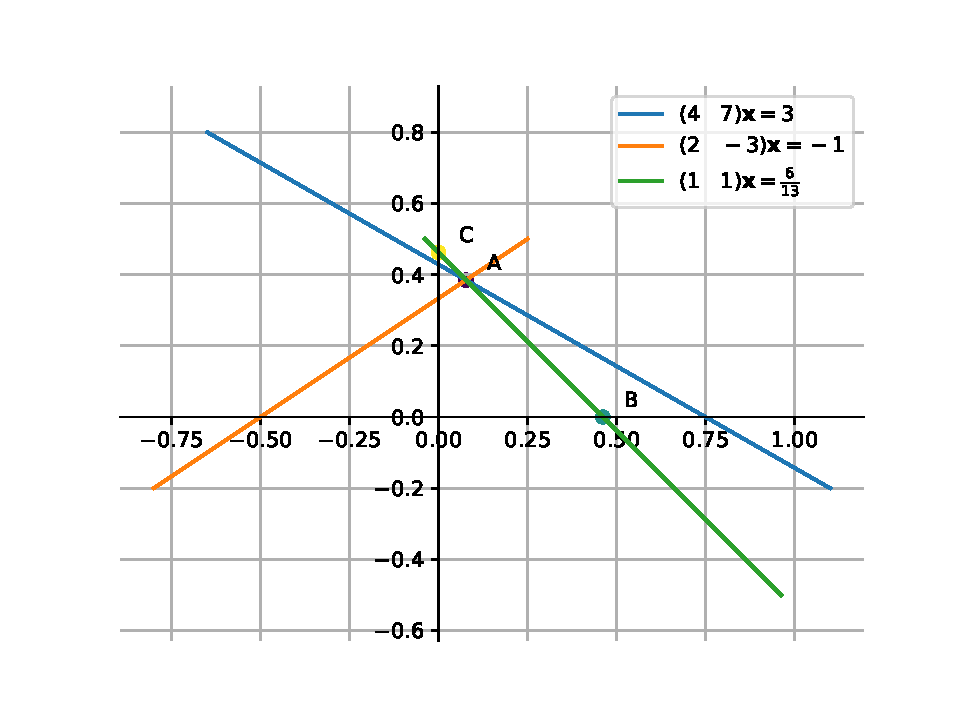
\includegraphics[width=0.75\columnwidth]{chapters/11/10/4/12/figs/fig.pdf}
    \caption{}
    \label{fig:enter-label}
\end{figure}
